% !TeX root = ../main.tex

\chapter{主要研究方法及技术路线}

\section{现有工具漏洞检测能力}

在开始进行实验之前,我们需要对现有工具的检测能力进行充分地调研。只有在了解现有工具的检测能力、检测特点的情况下,我们才能开始进行漏洞标准库的构建和新工具的研发工作。为此,我们调研了当下对Solidity的研究工作,有的工作来自于商业团队,有的来自于学术团队;有的工具已经开源,并具备一定的社区影响力,有的工具发表于计算机顶级国际会议,带来了巨大的科研价值。发表于国际会议的工作,有的没有开源,对于这些没有开源的工作,虽然有论文做详细的说明,但由于不能获取到源代码,我们没办法对系统的内核做更深一步的分析,所以这些工具尽管有一定的学术影响力,我们也只能放弃。对于已经开源的工作,有些工具的开发逻辑不够严谨,或者相关文档不够完备,这些工具我们虽然能取得它们的源代码,但由于无法清晰地分析系统实现,故这些工具我们也无法很好地去分析他们的检测原理和检测能力。综上,在经过我们的筛选后,我们对如下工具在主要漏洞上的检测能力做出了总结,并和我们的系统\textsc{Athena}做比较列于表\ref{tab:detection_capability}。

\begin{table}
  \centering\small
  \caption{现有工具对于主要漏洞的检测能力总结}
  \begin{tabular}{cccccc}
    \toprule
    % after \\: \hline or \cline{col1-col2} \cline{col3-col4} ...
     & \textsc{Slither} & \textsc{Oyente} & \textsc{Smartcheck} & \textsc{Securify} & \textsc{Athena} \\
     \midrule
    可重入漏洞 & $\checkmark$ & $\checkmark$ & $\times$ & $\checkmark$ & $\checkmark$ \\
    意外异常漏洞 & $\checkmark$ & $\times$ & $\checkmark$ & $\times$ & $\checkmark$ \\
    低级调用漏洞 & $\checkmark$ & $\times$ & $\checkmark$ & $\times$ & $\checkmark$ \\
    自毁漏洞 & $\checkmark$ & $\times$ & $\times$ & $\times$ & $\checkmark$ \\
    \bottomrule
  \end{tabular}
  \label{tab:detection_capability}
\end{table}

上表所列的工具皆为静态分析工具,其中\textsc{Oyente}主要使用符号执行分析技术;\textsc{Securify}主要把代码转换成Datalog语言,并使用\textsc{Souffle}进行分析。\textsc{Slither}和\textsc{Smartcheck}采用的是传统的静态分析技术,即通过分析源代码得到程序的控制流图,并在控制流图上用预先设定好的匹配规则去寻找漏洞。从表中不难看出,使用传统静态分析技术的工具分析能力都比较不错,\textsc{Slither}支持我们提及的所有漏洞的检测,\textsc{Smartcheck}不支持两个漏洞的检测;而使用符号执行分析技术,包括使用其他静态分析技术的工具,对主要漏洞的支持都不太好,甚至只支持一个漏洞的检测。值得一提的是,这两个工具\textsc{Oyente}和\textsc{Securify}皆是在源代码编译之后产生的字节码上进行软件分析的,字节码的分析提供的信息更少,相比之下\textsc{Slither}和\textsc{Smartcheck}都是对源代码或者中间语言进行分析,故我们推测是由于技术路线的差异造成它们在不同漏洞上的分析难度不同,也就没办法支持所有漏洞的分析任务。

\section{使用克隆分析技术寻找漏洞代码}

在克隆代码分析技术中,按照代码相似的不同程度,我们可以把代码划分为以下几种克隆层次:
\begin{itemize}
  \item \textbf{第一类克隆:完全克隆。}这种克隆下层次下的相似代码之间完全相似,没有任何差异。
  \item \textbf{第二类克隆:重命名克隆。}这种克隆层次下的代码之间绝大部分相似,在类型、标识符、注释、空格之间有些许差异。
  \item \textbf{第三类克隆:重构克隆。}这种克隆层次下的相似代码之间具有结构层次的不同,例如缺少部分语句,多出部分语句,语句顺序不同等等。
  \item \textbf{第四类克隆:语义克隆。}这种克隆层次下的相似代码之间可能完全不同,但他们具有相同的语义,实现了相同的功能或流程。
\end{itemize}
从克隆层次的分类我们可以看出,第一类克隆和第二类克隆不涉及代码结构上的变化,因而能用比较简单的技术进行分析。在Kamiya等人的工作中\cite{ccfinder},使用了基于标记的克隆分析技术来寻找克隆代码,将代码的关键部分转换为标记,再在标记上进行分析寻找。由于前两类克隆代码的分析并没有什么挑战,因此现在已经有很多这方面的工作。对于第三类克隆,因为代码之间出现了语句结构的差异,例如多的语句,少的语句等等,直接借助基于标记的克隆分析技术来寻找克隆代码可能会遇上很多困难。为了解决这一问题,有人提出了提取代码特征转换成特征向量,并在高维空间进行比较的办法\cite{deckard},也有的工作提出使用软件的控制流图进行语句结构的比较\textcolor{red}{Add citation here}。而对于第四类克隆的分析,仍然是当前软件工程学界的一个有挑战的课题。有的工作提出使用深度学习算法进行代码语义的提取\textcolor{red}{Add ICST citation},但仍有很大的局限性如学习算法的数据集匮乏,很难找到数量充足且质量上乘的训练材料。因此,在讨论克隆分析技术时,我们主要解决的是寻找前三类克隆的相似代码的问题。

针对以上三种代码克隆等级,之前的工作提出了很多不同粒度的解决方案:
\begin{enumerate}
  \item \textbf{基于标记粒度的克隆分析技术:}使用基于标记力度的克隆分析技术试图使用将代码语句转换成标记序列,然后再在标记序列上比较相似度。这其中最出名的工作有CP-Miner\cite{cpminer}。CP-Miner解析了程序代码,并使用了“最频繁子序列挖掘”算法对代码生成的标记序列进行比较。这个算法由CloSpan\cite{clospan}这篇工作提出。多亏了CloSpan这篇工作在改进算法运行效率方面的贡献,CP-Miner可以在大规模代码,如Linux内核代码下仍保持了较低的内存占用。但是,CP-Miner的运行时间复杂度在最坏情况下为$\mathcal{O}(n^{2})$,$n$为代码行数,运行耗时较长。除开在大规模代码下的效率问题,CP-Miner也容易产生很多误报,这个是由于他们激进的代码抽象策略及有筛选的遗产算法导致的。虽然CP-Miner的开发者认为CP-Miner在数据集上的表现不错,但很明显CP-Miner并没有在漏洞代码检测这项任务上有足够的可靠行。
  \item \textbf{基于代码行粒度的克隆分析技术:}在ReDeBug\cite{redebug}中,分析系统将代码行的集合作为处理单元。系统驱使一个$n$行($n$默认为4)的窗口在源代码中滑动,并在每个窗口上使用三种不同哈希函数。该系统通过对比两文件各窗口的哈希值来计算文件之间的相似程度。虽然ReDeBug的这个特性使它能够检查一些第三类克隆的克隆代码,但它却无法检查那些第二类克隆,即变量名或者数据类型有变化的克隆代码。因此,ReDeBug会漏掉很多有漏洞但差异很小的克隆代码。更进一步,使用基于代码行粒度的克隆分析技术会导致上下文信息被局限一个很小的范围内,并最终导致引入了很多的误报。同时,ReDeBug需要花费大量的时间去处理源代码文件并建立哈希库,性能表现欠佳。
  \item \textbf{基于函数粒度的克隆分析技术:}SourcererCC\cite{sourcerercc}使用了基于函数粒度的克隆分析技术,试图来检测第三类克隆的克隆代码。它使用了标记集的检测技术解析了所有的函数,并针对每个函数的标记集建立了检索目录;然后,它寻找两个函数间相同的标记,并使用了\emph{Overlap}函数计算这两个函数之间的相似度。如果这个相似度超过了人为预先确定的一个阈值,则判断在这两个函数之间存在代码克隆现象。该系统在实现时,为了减少相似度的计算次数,对标记按出现的频数进行权重计算,出现频数高的标记获得较高权重,对持有较高权重的标记进行计算。但是,在权衡检测第三类克隆代码的能力与检查漏洞的能力时,SourcererCC对与漏洞代码的检测能力受到了很大的限制。在很多情况下,打过补丁的代码(安全代码)与未打补丁的代码(漏洞代码)之间的差距非常小,甚至只有一个\codeff{if}语句的差距,SourcererCC也无法检测这些漏洞代码。

      Yamaguchi等人提出使用漏洞推导的方法\cite{vul-extrapolation}来分析第四类克隆,即语义克隆的代码。他们分析函数的抽象语法树,并提取语法树的特征并将其嵌入向量空间中;在完成提取工作后,他们对高维向量使用奇异值分解来获取函数的结构信息。虽然他们的方法具备了检测一定程度的第四类克隆的能力,但是他们的系统运行流程有太多的时间和空间消耗,并且在论文中他们也没有明确给出这种技术的准确程度。

      我们必须指出,在使用高级别的代码抽象技术(标记序列,语法树)来分析克隆代码可能对分析代码克隆是有帮助的,但他们不足以准确地分析相似的漏洞代码,因为这些漏洞的语境通常会非常复杂。
  \item \textbf{基于文件粒度的克隆分析技术:}DECKARD\cite{deckard}对每个源代码文件都分别构建了抽象语法树,并从文件的抽象语法树上提取了特征向量,再在特征向量上使用欧几里得距离来进行聚类,经过聚类,欧氏距离较近的文件则被判断为克隆代码文件。这种基于语法树的方法需要大量的执行时间,因为子图同构是一个著名的NP完全问题。更进一步说,DECKARD并没有保证足够的扩展性,在面对大数据集时表现差强人意,同时,DECKARD也带来了很高的误报率,这也说明具有相同语法树结构的代码片段可能不是克隆代码。

      FCFinder\cite{fcfinder}去除了代码的注释、重复空格、换行,再对代码用MD5算法计算哈希值。它建立了一个哈希表,表的键值为文件名,数值为对应文件的哈希值。如果发现有文件的哈希值重复,则判断这几个文件为克隆代码文件。相比于DECKARD,FCFinder具有了良好的可扩展性。再FreeBSD软件上的克隆检测上,耗时更少,同时保持了一定的准确率。 可是,和DECKARD一样,它也不能很好地检测高度相似但具有微笑不同的克隆代码。
  \item \textbf{混合粒度的克隆分析技术:}有一些工作使用了几种不同粒度的克隆分析技术。VulPecker\cite{vulpecker}是一个能自动检查漏洞的软件分析系统。它给漏洞加上了事先定义好的特征,再根据代码的实际情况算则合适的代码相似度算法(如最长公共字串算法)计算代码相似度。在这个分析技术的帮助下,它找到了40个未被NVD(National Vulnerability Database)记录在案的漏洞。可是,这个系统在大量代码的情况下耗时过长,无法应对大量代码的检测任务。
\end{enumerate}

综上所述,对于不同粒度不同情况下的克隆代码分析,之前的工作做出了相当的努力。同时,我们也不难看出,要达成使用克隆分析技术来寻找代码漏洞的目标,我们不仅要保证我们的检测器具备一定的扩展性,以应对检测大量的代码的情况;其次我们也应该选用合理的代码抽象代码,来提取不同漏洞的特征,借助提取的特征来匹配相似的代码片段;最后,代码相似度计算算法的选择对分析克隆代码的能力至关重要,我们应该合理地选择代码相似度的计算算法。

\section{在智能合约软件上使用克隆分析技术的可行性}

在上一个部分我们调研了现有的软件克隆分析技术在不同的软件克隆等级上的效果和优缺点,我们也提出了要实现使用克隆分析技术去寻找漏洞代码,不仅要谨慎选择相似度算法,也必须保证系统即使在面对大量代码时也能维持较快的检测速度。但是,目前还没有工作在智能合约上使用克隆分析技术去寻找漏洞代码,因此,在这一部分,我们将证明在智能合约软件上使用克隆分析技术是可行的。

\subsection{智能合约代码相似度观察}
在我们观察了大量的智能合约软件代码过后,我们发现,在以太坊平台上存在着大量的代码克隆现象。在我们从Etherscan\footnote{一个提供智能合约数据及分析服务的网站。}上爬取了接近十万的智能合约代码,在使用最长公共字串来计算代码间相似度之后我们发现,统计代码相似度层级如下图\ref{fig:similarity}所示。
\begin{figure}[htbp]
\vspace{+2mm}
  \centering
  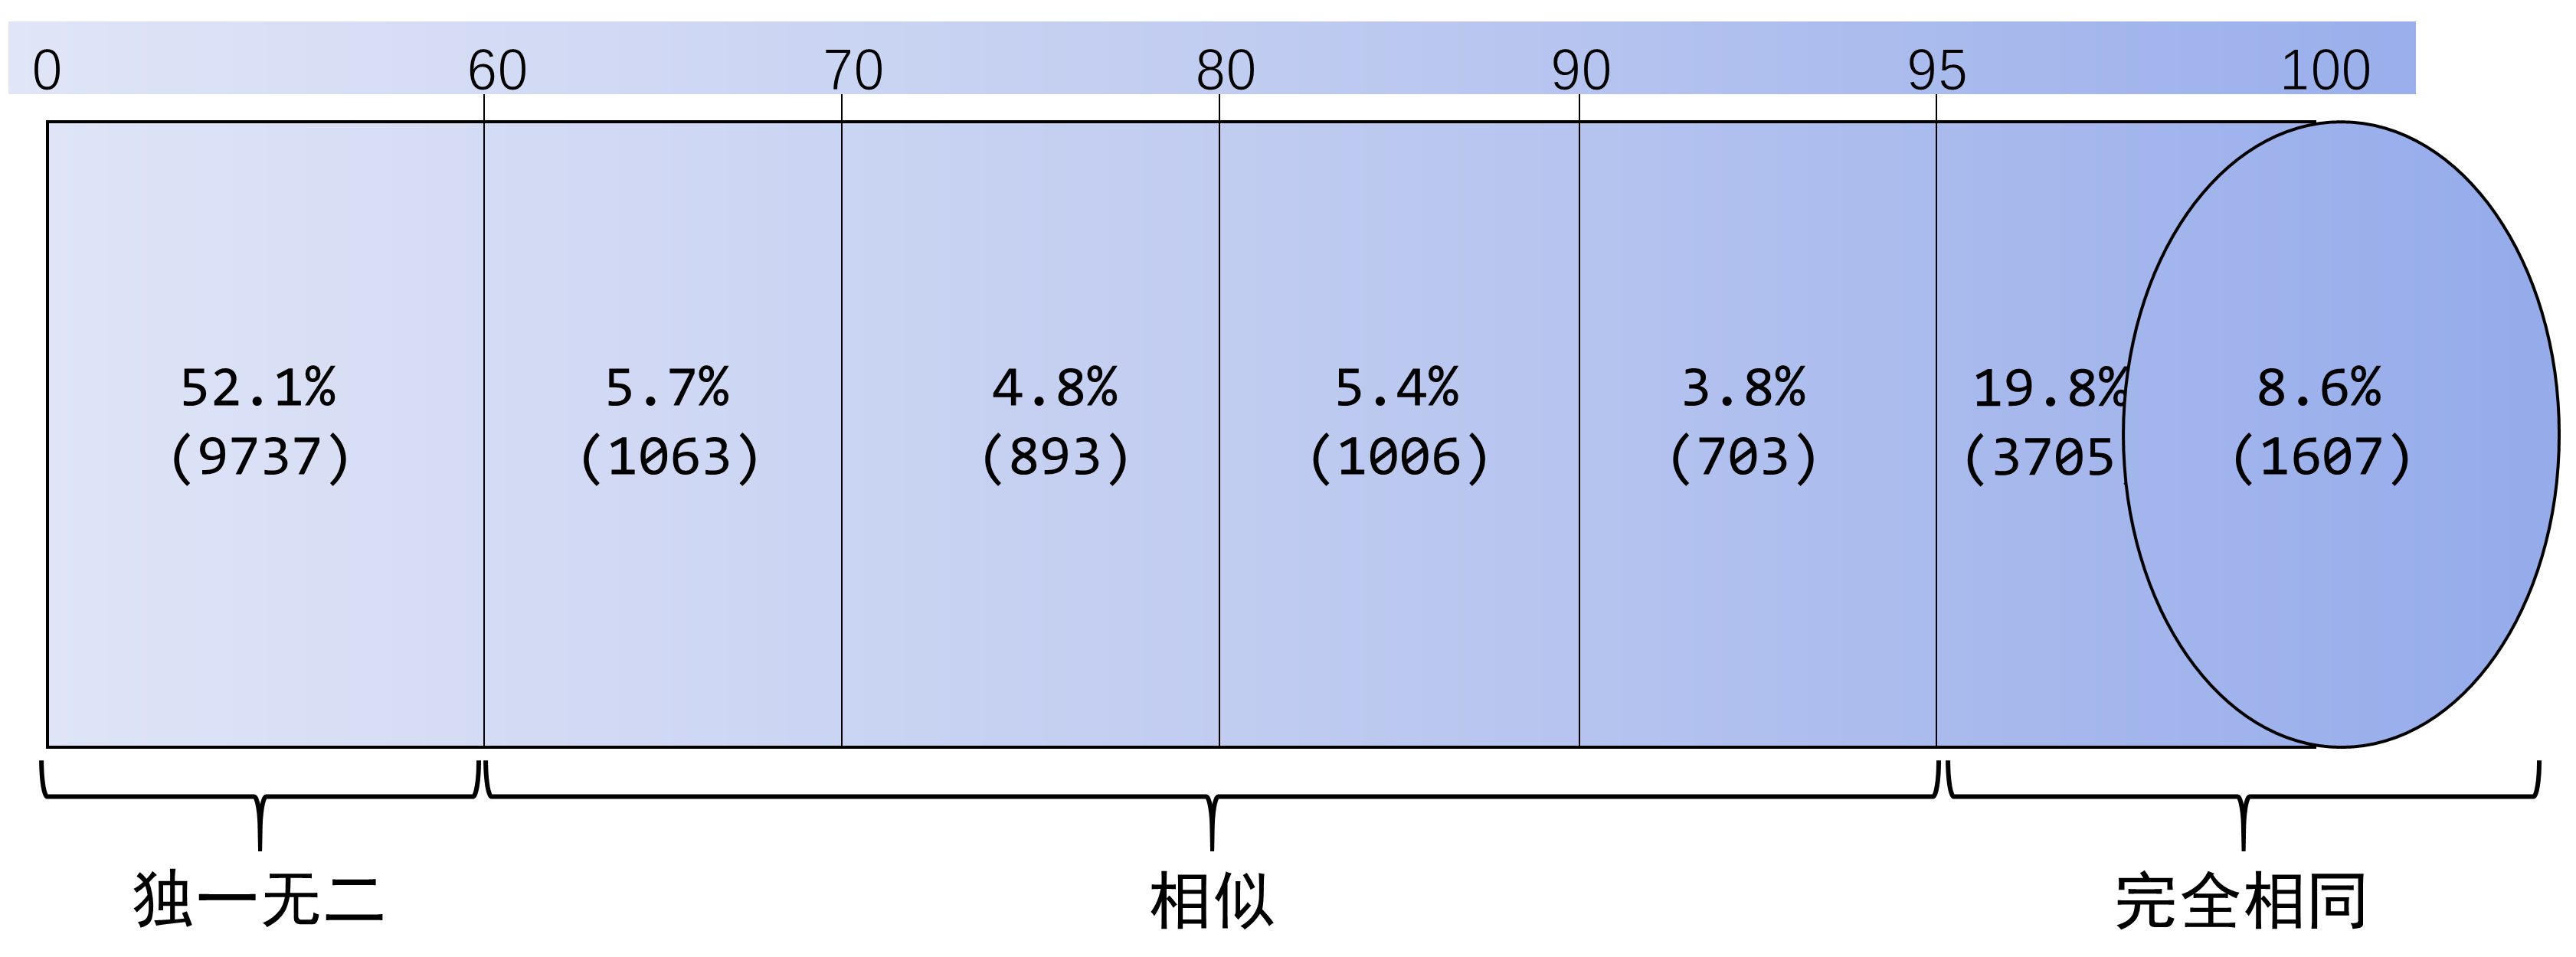
\includegraphics[width=0.9\textwidth]{figures/similarity.png}
  \caption{智能合约代码相似度统计}
  \label{fig:similarity}
\vspace{-5mm}
\end{figure}
我们可以明显看出,大部分智能合约软件内部存在着代码克隆现象,我们推测这是由于Solidity代码无法引用代码引起的。很多智能合约软件直接复制已经存在的软件代码,稍加改动,如修改了交易地址,甚至不改动就添加到自己的代码中,参与自己软件的运行过程。很明显,这虽然方便了开发者,减轻了开发任务,但是直接拷贝代码的行为容易在无意间引入漏洞。在一个存在很多克隆代码的平台,要保证软件的平均安全等级是很困难的。Solidity研究团队推荐开发者拷贝或使用经过官方团队审计的接口代码,但是不推荐开发者拷贝其他任何代码。
\begin{figure}[H]
    \centering
    \begin{subfigure}{.5\linewidth}
    \centering
    \begin{minipage}{1.0\linewidth}
    \begin{lstlisting}
    function refundAll() public {
    for(uint x; x < refundAddresses.length; x++) {
    require(refundAddresses[x]);
    }
    }
    \end{lstlisting}
    %\caption{test}
    \end{minipage}
    \caption{相似代码示例}
    \end{subfigure}
    \quad
    \begin{subfigure}{.5\linewidth}
    \centering
    \begin{minipage}{1.0\linewidth}
    \begin{lstlisting}
    contract gamble{
    ...
    public suicidal(address target) public {
    selfdestruct(target);
    }
    }
    \end{lstlisting}
    %\caption{test}
    \end{minipage}
    \caption{相似代码示例}
    \end{subfigure}
    \caption{相似代码示例}
    \label{fig:similar_code}
\end{figure}

\subsection{智能合约克隆分析技术探究}
针对以太坊平台如此严重的代码克隆现象,我们提出使用代码克隆分析技术来寻找漏洞的方法。在VUDDY\cite{vuddy}这篇工作中,研发团队使用了根据漏洞代码的语法特征提取了漏洞的抽象表示,再通过相似度计算算法来寻找漏洞代码。VUDDY的这种技术,是从漏洞本身出发,寻找与漏洞相似代码的一种技术。这种方法具备良好的可扩展性,在寻找大量相似代码时也能保证令人满意的速度,在VUDDY的论文中,开发团队使用VUDDY完成了数以亿计行的代码的漏洞检测工作,并成功申请了数十个CVE。VUDDY的工作给了我们启发,在智能合约上,我们需要使用一种足够巧妙的方法去提取漏洞的抽象表现形式,抽象程度不能太高或者太低,太高会误报很多漏洞代码,太低则会漏掉很多真实的漏洞代码;我们还需要使用足够巧妙的代码相似度算法去计算代码之间的相似度,这种相似度计算方法必须和代码的抽象表现形式结合,不能有太高的时间复杂度;最后,我们需要对系统报告的漏洞做一定程度的人工分析,虽然在严谨的实验中,人工的行为容易带来实验结果的偏差,但是我们参与实验的检查人员都是智能合约、区块链及软件工程方面的领域专家,可以尽可能减少人工介入带来的偏差。那些经过人工检查,或者被系统报告有漏洞的代码,我们会用来不断地改进我们系统的检测能力,并建立漏洞标准库。

\subsection{结合克隆分析技术与字节码分析技术}
我们的系统不仅提供对智能合约源代码的漏洞检测功能,也能完成对字节码的反汇编任务以及控制流图分析。\textsc{Oyente}\cite{oyente}在字节码的基础上,使用了反汇编技术结合控制流图分析,并加上了符号执行分析技术,实现了漏洞的检测。无独有偶,之后的符号执行技术如\textsc{SCompile}\cite{scompile},\textsc{Manticore}\cite{manticore}也是在字节码上使用了符号分析技术,并结合自己确定的漏洞规则来进行检测。在我们的系统中,我们并不打算在字节码上加入符号分析技术并对字节码进行漏洞检测,我们只提供对字节码的代码结构静态分析,这是因为经过我们的广泛调研,如今字节码的反编译技术及语义解析技术并不是很成熟,我们觉得不足以支撑实现一个具有一定准确率的漏洞检测系统;其次,加入符号分析技术的工作量过大,超出了我们这篇论文的研究范畴,我们也希望相关同僚在字节码的漏洞分析检测技术上取得进一步的突破。

\subsection{漏洞检测系统结构设计}
我们给出了我们整体的系统结构,如图\ref{fig:system_diagram}所示。系统使用智能合约软件作为输入,分析结果及标准数据库作为输出。在系统的开始,会对输入的智能合约软件做相关检测,如果输入的智能合约软件为源代码形式,则进行源代码分析及进一步的漏洞检测;如果输入的智能合约软件为字节码形式,则对字节码进行反汇编,并将得到的汇编码作为输入进行控制流图分析,最后输出简单的分析结果。在源代码结束控制流图分析之后,我们将对软件进行漏洞签名匹配。漏洞签名是经过我们智能合约领域专家总结得出的一套漏洞模板,并进行一定程度的抽象。再之后,我们用相似度算法计算漏洞签名与输入的控制流图进行相似度计算,如果得到的相似度高于我们设定好的阈值,我们就判断这是一个可疑的漏洞代码,我们将把这段代码保存并交由我们领域专家进行进一步检查。加入人工检查的目的是为了漏洞检测系统的公平公正,当下的对于智能合约漏洞检测的论文中对于漏洞的定义并不一致,且尚没有一个高度完备的工作能囊括所有的漏洞形式,因此,为了方便标准库构建和系统的优化,我们需要专家进行一定程度的人工干预,对系统的检测结果进行二次检测。如果专家检查到了系统的误报,说明我们总结的漏洞签名仍有不完备的地方,我们将根据误报的漏洞形式进一步完善系统的漏洞签名。漏洞签名的完善我们将根据漏洞的误报形式来决定,并不是所有的误报我们都要进行改进。这也是进行人工干预的优点,可以选择需要改进的地方进行恰当的改进。最后,对于那些系统正确判断的软件漏洞,我们将把漏洞代码加入漏洞库。漏洞库是我们标准库构建工作的结晶,经过不断修缮也能给后续的智能合约软件分析工作带来长远的便利。出于人道主义和安全考虑,我们并不会公开我们漏洞库的所有漏洞,但是我们会匿名掉关键信息并展示部分漏洞代码作为案例分析的一部分。随着和漏洞代码的作者联系不断进行,如果软件作者已经做出相关回应,修复了漏洞,我们也会在将来公开更多的漏洞代码用作学习和警示。
\begin{figure}[b]
\vspace{+2mm}
  \centering
  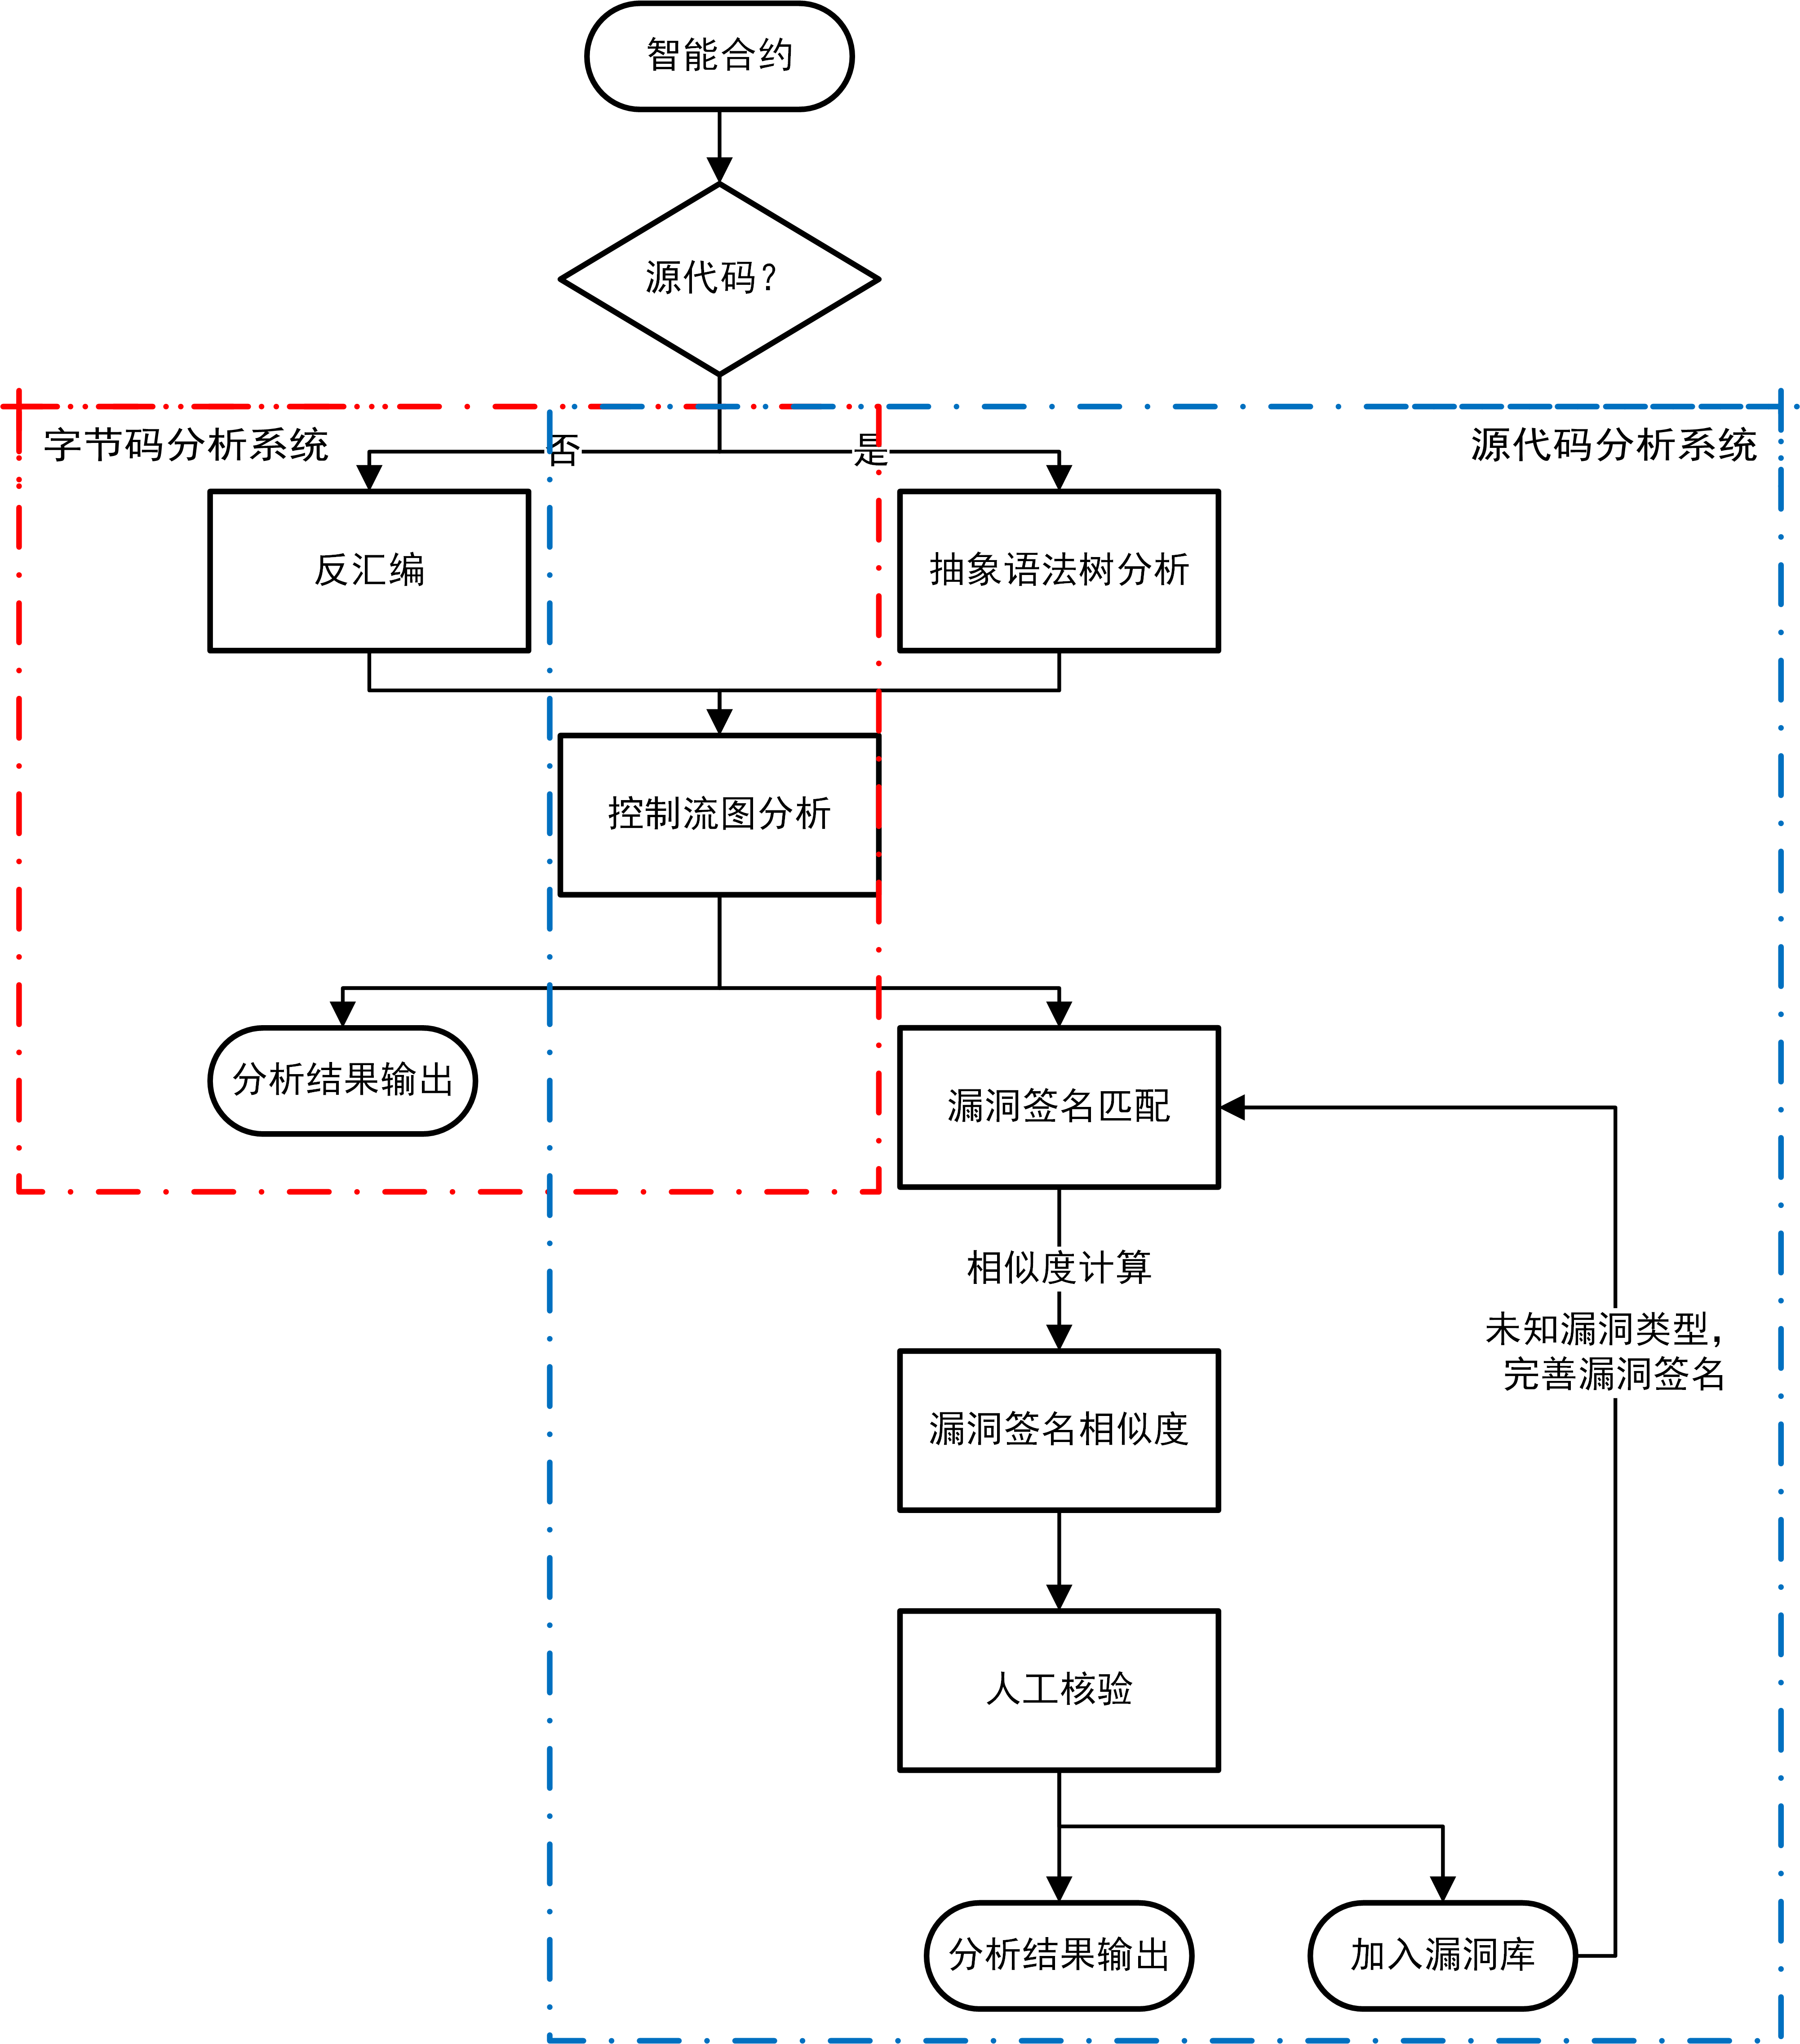
\includegraphics[width=0.8\textwidth]{figures/system_diagram.png}
  \caption{漏洞检测系统结构设计图}
  \label{fig:system_diagram}
\vspace{-5mm}
\end{figure}